\chapter{Arhitektura i dizajn sustava}
		
		\textbf{\textit{dio 1. revizije}}\\

		\textit{ Potrebno je opisati stil arhitekture te identificirati: podsustave, preslikavanje na radnu platformu, spremišta podataka, mrežne protokole, globalni upravljački tok i sklopovsko-programske zahtjeve. Po točkama razraditi i popratiti odgovarajućim skicama:}
	\begin{itemize}
		\item 	\textit{izbor arhitekture temeljem principa oblikovanja pokazanih na predavanjima (objasniti zašto ste baš odabrali takvu arhitekturu)}
		\item 	\textit{organizaciju sustava s najviše razine apstrakcije (npr. klijent-poslužitelj, baza podataka, datotečni sustav, grafičko sučelje)}
		\item 	\textit{organizaciju aplikacije (npr. slojevi frontend i backend, MVC arhitektura) }		
	\end{itemize}

	
		

		

				
		\section{Baza podataka}
			
			\textbf{\textit{dio 1. revizije}}\\
			
		\textit{Potrebno je opisati koju vrstu i implementaciju baze podataka ste odabrali, glavne komponente od kojih se sastoji i slično.}
		
			\subsection{Opis tablica}
			
				
				\begin{longtabu} to \textwidth {|X[6, l]|X[6, l]|X[20, l]|}
					
					\hline \multicolumn{3}{|c|}{\textbf{Korisnik}}	 \\[3pt] \hline
					\endfirsthead
					
					\hline \multicolumn{3}{|c|}{\textbf{Korisnik }}	 \\[3pt] \hline
					\endhead
					
					\hline 
					\endlastfoot
					
					\cellcolor{LightGreen}ID${\_}$Korisnik & SERIAL	& jedinstveni identifikator korisnika 	 	\\ \hline
					ime & VARCHAR	&  ime korisnika	\\ \hline 
					prezime & VARCHAR	& prezime korisnika 		\\ \hline
					email & VARCHAR & e-mail adresa korisnika  \\ \hline 
					lozinka	& VARCHAR & hash lozinke 	\\ \hline 
					uloga	& VARCHAR & uloga korisnika (administrator ili registrirani korisnik)  	\\ \hline 
					\cellcolor{LightBlue} geolokacija	& VARCHAR & geografska dužina i širina  	\\ \hline 
					
					
				\end{longtabu}
			
			
				\begin{longtabu} to \textwidth {|X[6, l]|X[6, l]|X[20, l]|}
					
					\hline \multicolumn{3}{|c|}{\textbf{Zahtjev}}	 \\[3pt] \hline
					\endfirsthead
					
					\hline \multicolumn{3}{|c|}{\textbf{Zahtjev }}	 \\[3pt] \hline
					\endhead
					
					\hline 
					\endlastfoot
					
					\cellcolor{LightGreen}ID${\_}$Zahtjev & SERIAL	&  jedinstveni identifikator korisnika	 	\\ \hline
					opis & VARCHAR	& opis zahtjeva 		\\ \hline 
					date & DATE	& datum do kada se treba izvršiti zahtjev  		\\ \hline
					vrijeme & TIME & vrijeme do kada se treba izvršiti zahtjev \\ \hline 
					status	& VARCHAR & status zahtjeva  	\\ \hline 
					\cellcolor{LightBlue} geolokacija	& VARCHAR &geografska dužina i širina    	\\ \hline 
					
					
				\end{longtabu}
			
			
				\begin{longtabu} to \textwidth {|X[6, l]|X[6, l]|X[20, l]|}
					
					\hline \multicolumn{3}{|c|}{\textbf{Lokacija}}	 \\[3pt] \hline
					\endfirsthead
					
					\hline \multicolumn{3}{|c|}{\textbf{Lokacija }}	 \\[3pt] \hline
					\endhead
					
					\hline 
					\endlastfoot
					
					\cellcolor{LightGreen}geolokacija & SERIAL	& geografska dužina i širina  	\\ \hline
					p${\_}$kod & INT	&  post kod		\\ \hline 
					drzava & VARCHAR	& naziv države 		\\ \hline
					naselje & VARCHAR & naziv naselja  \\ \hline 
					adresa	& VARCHAR & adresa na kojoj treba odraditi zahtjev	\\ \hline 	
					
				\end{longtabu}
			
			
			
				\begin{longtabu} to \textwidth {|X[6, l]|X[6, l]|X[20, l]|}
					
					\hline \multicolumn{3}{|c|}{\textbf{Aut${\_}$Zahtj${\_}$Izvr}}	 \\[3pt] \hline
					\endfirsthead
					
					\hline \multicolumn{3}{|c|}{\textbf{Aut${\_}$Zahtj${\_}$Izvr}}	 \\[3pt] \hline
					\endhead
					
					\hline 
					\endlastfoot
					
					\cellcolor{LightGreen}ID${\_}$Zahtjev & INT	& jedinstveni identifikator zahtjeva 	\\ \hline
					\cellcolor{LightBlue}ID${\_}$Autor & INT	& jedinstveni identifikator autora zahtjeva 	\\ \hline
					\cellcolor{LightBlue}ID${\_}$Izvrsitelj & SERIAL	& jedinstveni identifikator izvršitelja zahtjeva  	\\ \hline
				
					
					
				\end{longtabu}
			
				\begin{longtabu} to \textwidth {|X[7, l]|X[6, l]|X[20, l]|}
					
					\hline \multicolumn{3}{|c|}{\textbf{Kandidatura}}	 \\[3pt] \hline
					\endfirsthead
					
					\hline \multicolumn{3}{|c|}{\textbf{Kandidatura}}	 \\[3pt] \hline
					\endhead
					
					\hline 
					\endlastfoot
					
					\cellcolor{LightGreen}ID${\_}$Kandidatura & SERIAL	& jedinstveni identifikator kandidature 	\\ \hline
					godina & INT & godina kandidature  \\ \hline 
					\cellcolor{LightBlue}ID${\_}$Korisnik & INT	& jedinstveni identifikator korisnika 	\\ \hline
					
				\end{longtabu}
				
				
				\begin{longtabu} to \textwidth {|X[6, l]|X[6, l]|X[20, l]|}
					
					\hline \multicolumn{3}{|c|}{\textbf{Ocjena}}	 \\[3pt] \hline
					\endfirsthead
					
					\hline \multicolumn{3}{|c|}{\textbf{Ocjena }}	 \\[3pt] \hline
					\endhead
					
					\hline 
					\endlastfoot
					
					\cellcolor{LightGreen}ID${\_}$Ocjenitelj & INT	& jedinstveni identifikator ocjenitelja 	\\ \hline
					\cellcolor{LightGreen}ID${\_}$Ocjenjeni & INT	& jedinstveni identifikator ocjenjenog 	\\ \hline
					ocjena & INT	&  ocjena usluge		\\ \hline 
					komentar & VARCHAR	& komentar ocjenitelja 		\\ \hline
					
					
					
				\end{longtabu}
		
		
			\subsection{Dijagram baze podataka}
			
			%unos slike
			\begin{figure}[H]
				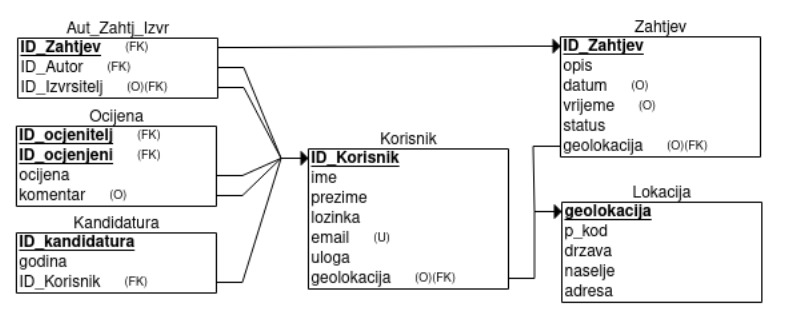
\includegraphics[scale=0.65]{slike/dijagram2.jpeg} %veličina slike u odnosu na originalnu datoteku i pozicija slike
				\centering
				\caption \newline E-R dijagram baze podataka
				\label{fig:promjene}
			\end{figure}
			
			\eject
			
			
		\section{Dijagram razreda}
		
			\textit{Potrebno je priložiti dijagram razreda s pripadajućim opisom. Zbog preglednosti je moguće dijagram razlomiti na više njih, ali moraju biti grupirani prema sličnim razinama apstrakcije i srodnim funkcionalnostima.}\\
			
			\textbf{\textit{dio 1. revizije}}\\
			
			\textit{Prilikom prve predaje projekta, potrebno je priložiti potpuno razrađen dijagram razreda vezan uz \textbf{generičku funkcionalnost} sustava. Ostale funkcionalnosti trebaju biti idejno razrađene u dijagramu sa sljedećim komponentama: nazivi razreda, nazivi metoda i vrste pristupa metodama (npr. javni, zaštićeni), nazivi atributa razreda, veze i odnosi između razreda.}\\
			
			\textbf{\textit{dio 2. revizije}}\\			
			
			\textit{Prilikom druge predaje projekta dijagram razreda i opisi moraju odgovarati stvarnom stanju implementacije}
			
			
			
			\eject
		
		\section{Dijagram stanja}
			
			
			\textbf{\textit{dio 2. revizije}}\\
			
			\textit{Potrebno je priložiti dijagram stanja i opisati ga. Dovoljan je jedan dijagram stanja koji prikazuje \textbf{značajan dio funkcionalnosti} sustava. Na primjer, stanja korisničkog sučelja i tijek korištenja neke ključne funkcionalnosti jesu značajan dio sustava, a registracija i prijava nisu. }
			
			
			\eject 
		
		\section{Dijagram aktivnosti}
			
			\textbf{\textit{dio 2. revizije}}\\
			
			 \textit{Potrebno je priložiti dijagram aktivnosti s pripadajućim opisom. Dijagram aktivnosti treba prikazivati značajan dio sustava.}
			
			\eject
		\section{Dijagram komponenti}
		
			\textbf{\textit{dio 2. revizije}}\\
		
			 \textit{Potrebno je priložiti dijagram komponenti s pripadajućim opisom. Dijagram komponenti treba prikazivati strukturu cijele aplikacije.}